\documentclass{exam}
\usepackage[utf8]{inputenc}
\usepackage{lmodern}
\usepackage{microtype}

% \usepackage[parfill]{parskip}
\usepackage[dvipsnames]{xcolor}
\usepackage{amsmath}
\usepackage{amsfonts}
\usepackage{amsthm}
\usepackage{siunitx}
\DeclareSIUnit\year{yr}
\DeclareSIUnit\foot{ft}
\DeclareSIUnit\litre{\liter}

\usepackage{skull}

\usepackage{pgfplots}
\usepgfplotslibrary{polar}
\pgfplotsset{compat=1.11}
\usepgfplotslibrary{statistics}
\usepackage{graphicx}
\usepackage{sidecap}
\sidecaptionvpos{figure}{c}
\usepackage{float}
\usepackage{gensymb}
\usepackage{tkz-euclide}
\usetkzobj{all}
\usepackage{commath}
\usepackage{hyperref}
\usepackage{enumitem}
\usepackage{wasysym}
\usepackage{multicol}
\usepackage{mathtools}
\usepackage{tcolorbox}
\usepackage{tabularx}
\usepackage[version=4]{mhchem}
\usepackage{changepage}
\usepackage{listings}
\lstset{basicstyle=\ttfamily\linespread{0.8}\small}

\renewcommand*{\thefootnote}{\fnsymbol{footnote}}

\newtheorem*{thm}{Theorem}
\newtheorem*{iden}{Identity}
\newtheorem*{lemma}{Lemma}
\newtheorem{obs}{Observation}
\theoremstyle{definition}
\newtheorem*{defn}{Definition}
\newtheorem*{ex}{Example}
\newtheorem{con}{Construction}
\newtheorem*{alg}{Algorithm}

\newtheoremstyle{break}
  {\topsep}{\topsep}%
  {\itshape}{}%
  {\bfseries}{}%
  {\newline}{}%
\theoremstyle{break}
\newtheorem*{bthm}{Theorem}

% russian integral
\usepackage{scalerel}
\DeclareMathOperator*{\rint}{\scalerel*{\rotatebox{17}{$\!\int\!$}}{\int}}

% \DeclareMathOperator*{\rint}{\int}

\pgfplotsset{vasymptote/.style={
    before end axis/.append code={
        \draw[densely dashed] ({rel axis cs:0,0} -| {axis cs:#1,0})
        -- ({rel axis cs:0,1} -| {axis cs:#1,0});
    }
}}

% \pointsinrightmargin
\boxedpoints
\pointname{}

\newcommand{\questioA}{\question[\texttt{\textbf{\color{Cerulean} A}}]}
\newcommand{\questioM}{\question[\texttt{\textbf{\color{PineGreen} M}}]}
\newcommand{\questioE}{\question[\texttt{\textbf{\color{WildStrawberry} E}}]}
\newcommand{\questioS}{\question[\texttt{\textbf{\color{Goldenrod} S}}]}
\newcommand{\questioO}{\question[\texttt{\textbf{\color{BurntOrange} O}}]}

\newcommand{\parA}{\part[\texttt{\textbf{\color{Cerulean} A}}]}
\newcommand{\parM}{\part[\texttt{\textbf{\color{PineGreen} M}}]}
\newcommand{\parE}{\part[\texttt{\textbf{\color{WildStrawberry} E}}]}
\newcommand{\parS}{\part[\texttt{\textbf{\color{Goldenrod} S}}]}
\newcommand{\parO}{\part[\texttt{\textbf{\color{BurntOrange} O}}]}

\newcommand{\subparA}{\subpart[\texttt{\textbf{\color{Cerulean} A}}]}
\newcommand{\subparM}{\subpart[\texttt{\textbf{\color{PineGreen} M}}]}
\newcommand{\subparE}{\subpart[\texttt{\textbf{\color{WildStrawberry} E}}]}
\newcommand{\subparS}{\subpart[\texttt{\textbf{\color{Goldenrod} S}}]}
\newcommand{\subparO}{\subpart[\texttt{\textbf{\color{BurntOrange} O}}]}

\newcommand{\mainHeader}[2]{\section*{NCEA Level 2 Mathematics\\#1. #2}}
\newcommand{\mainHeaderHw}[2]{\section*{NCEA Level 2 Mathematics (Homework)\\#1. #2}}
\newcommand{\seealso}[1]{\begin{center}\emph{See also #1.}\end{center}}
\newcommand{\drills}[1]{\begin{center}\emph{Drill problems: #1.}\end{center}}
\newcommand{\basedon}[1]{\begin{center}\emph{Notes largely based on #1.}\end{center}}

\begin{document}

\mainHeaderDiffHw{10}{Inverse Functions}
\subsection*{Reading}
\goandwatch{https://www.youtube.com/watch?v=J-BdwKtsnYs}

There is an important theorem in analysis that is relatively easy to guess is true within the limited range of functions we
have looked at: the inverse function theorem. The inverse function theorem essentially states that if a function is continuous
at some point, and if its derivative exists and is continuous at that point, then the function has an inverse around that point.

For example, consider the curve $ x^4 + y^4 = 16$ graphed here. Notice that the curve fails the horizontal line test everywhere (so
does not have an inverse) and fails the vertical line test everywhere (so is not even a function).
\begin{center}
  
\includegraphics[width=0.2\linewidth]{implicit15}
\end{center}

This curve can be represented by the function $ \theta \mapsto (\pm4\sqrt{\cos \theta}, \pm4\sqrt{\sin \theta}) $ for $ 0 \leq t < 2\pi $. Let's
zoom in and look at the first quadrant.
\begin{center}
  \fbox{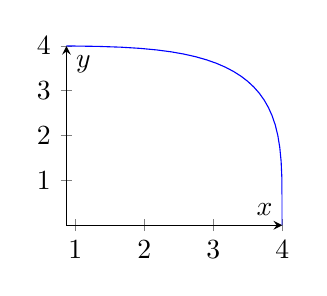
\begin{tikzpicture}
    \begin{axis}[
      scale = .4,
      axis lines = center,
      xlabel = $ x $,
      ylabel = $ y $
    ]
      \addplot[domain = 0:2*pi, color = blue, samples=100] ({4*(cos(deg(x)))^(1/2)}, {4*(sin(deg(x)))^(1/2)});
    \end{axis}
  \end{tikzpicture}}
\end{center}
In particular, if we restrict ourselves to this region then the curve is both a function \emph{and} is 1-1 --- so this section of
the function has an inverse. This occurs because each $ y$-value corresponds to a particular $ \theta$-value in this segment, and then
we can (using our parameterisation) map that $ \theta$-value onto the corresponding $ x$-value.


\subsection*{Questions}
\begin{questions}
  \question Find the derivatives with respect to $ x $:
    \begin{parts}
      \part $ y = \tan^{-1} (x^2) $
      \part $ \tan f(x) = x $
      \part $ g(x) = \arctan(\arcsin \sqrt{x}) $
    \end{parts}
  \question Show that
    \begin{displaymath}
      \od{}{x} \left( \frac{1}{2} \tan^{-1} x + \frac{1}{4} \ln\frac{(x + 1)^2}{x^2 + 1} \right) = \frac{1}{(1 + x)(1 + x^2)}
    \end{displaymath}
  \question Prove that $ \od{}{x} \cot^{-1} x = -\frac{1}{x^2 + 1} $.
\end{questions}

\end{document}
